\section{\textit{Queue-Based Load Leveling Pattern}}

Sebuah layanan dalam satu sistem seringkali bertugas untuk mengerjakan sesuatu dan memanggil layanan lain. Dalam kasus ini, terdapat kemungkinan munculnya masalah kinerja dan keandalan ketika layanan mengalami beban yang tinggi. Keadaan ini dapat menciptakan situasi \textit{backpressure}.

Dalam konteks perangkat lunak, \textit{backpressure} dapat didefinisikan sebagai \textit{resistance or force opposing the desired flow of data through software} \parencite{backpressureExplained}. Selain melakukan penyesuaian pada sumber daya sistem, terdapat tiga strategi yang dapat digunakan untuk menangani \textit{backpressure}, yaitu:

\begin{enumerate}
    \item Mengurangi kecepatan \textit{producer} mengirimkan pesan.
    \item Menggunakan \textit{buffer} untuk sementara mengakumulasikan pesan.
    \item Membuang (\textit{drop}) sebagian pesan yang diterima.
\end{enumerate}

\textit{Queue-based load leveling} merupakan \textit{design pattern} yang menyelesaikan masalah ini dengan menggunakan \textit{queue} yang bertindak sebagai \textit{buffer} antara pekerjaan atau pesan dengan sebuah layanan sehingga beban dapat dikontrol dan layanan tetap berjalan dengan stabil \parencite{queueLoadLeveling}.

\begin{figure}[ht]
    \centering
    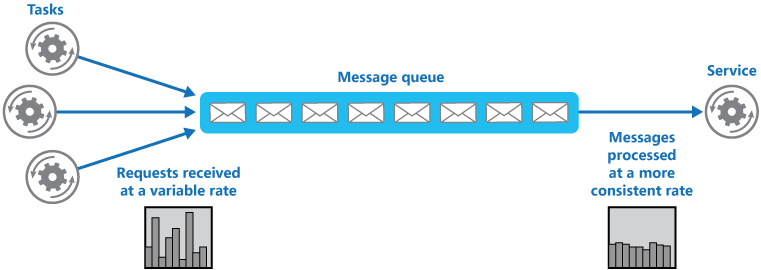
\includegraphics[width=0.8\textwidth]{resources/chapter-2/queue-based-load-leveling-pattern.png}
    \caption{\textit{Queue-Based Load Leveling Pattern Example} \parencite{queueLoadLeveling}}
    \label{fig:queue-based-load-leveling-pattern}
\end{figure}

Penggunaan \textit{queue} memisahkan pekerjaan dengan pekerja, sehingga pekerja dapat menangani pekerjaan berdasarkan kecepatannya terlepas dari banyaknya pekerjaan yang bertambah seiring dengan berjalannya waktu. Pola ini memiliki berbagai keuntungan, seperti meningkatkan \textit{availability}, memaksimalkan \textit{scalability}, dan membatasi biaya atau penggunaan sumber daya. Meskipun begitu, penggunaan pola ini akan meningkatkan latensi, terlebih lagi apabila pekerjaan yang dikirimkan jauh lebih besar daripada kapasitas pemrosesan pekerjaan pada sistem.